\chapter{Plane-wave Representation of Two-dimentional Fields}
\label{ch:pw2d}
Plane waves are exact solutions of Maxwell's fundamental field equations. Maxwell's equations are linear, provided the medium itself is linear (that is, the electrical properties of the medium such as its permittivity and permeability are independent of the electric and magnetic field). Hence the principle of linear superposition applies, and the superposition of individual plane waves traveling in different directions in the medium constitutes an exact solution.

Our ultimate goal is to study the diffraction of electromagnetic waves in realistic, three-dimensional situations. But it is much easier to introduce the underlying concepts and techniques in two dimensions. Hence this chapter is devoted to building up a picture of two-dimensional fields in term of individual plane of this representation. In the following chapter it will then to be possible to extend the representation to three dimensions, concentrating on the inevitably increased complexity of the mathematical while taking the underlying concepts for granted.

\section{Plane Waves}
\label{sec:plwa}
We begin by listing the properties of homogeneous plane electromagnetic waves. These will be familiar to most readers. But if they are not, a derivation based on transmission-line theory can be found in Appendix \ref{ch:tranline}.

A plane electromagnetic waves, of single-frequency time dependence $\exp(j\omega t)$, traveling in a uniform, isotropic an lossless open region, has the following properties:
\begin{figure}[htbp]
	\begin{center}
		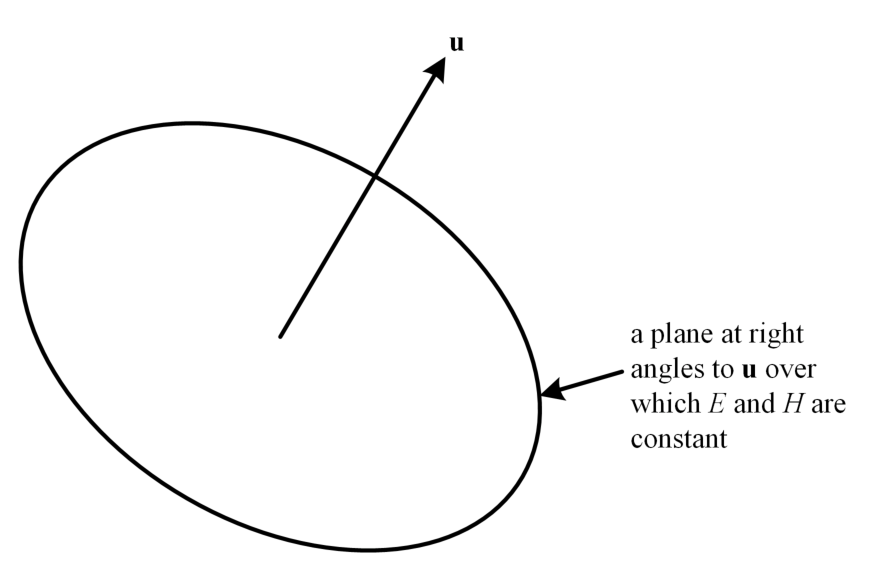
\epsfig{height=2.5in,file=Figs/pw2d/pwtrav.eps}
	\end{center}
	\caption{A plane wave traveling in the direction of $\mathbf{u}$.}
	\label{fig:pwtrav}
\end{figure}
\begin{itemize}
	\item [(a)]
	It is characterized by a single direction, such as that denoted by the unit $\mathbf{u}$ in Fig. \ref{fig:pwtrav}. This direction is the direction of propagation of the plane wave.
	\item [(b)]
	Over planes at right angles to $\mathbf{u}$ the phasor electric and magnetic fields, $E$ and $H$, are constant in both amplitude and phase.
	\item [(c)]
	The complex amplitude $E$ and $H$ are related to each other by the proportionality
	\begin{equation}
	E=ZH
	\end{equation}
	in which the constant $Z$ is the characteristic (or plane-wave) impedance of the medium. In the SI system, the units of $E$ are volts per meter and those of $H$ are amperes per meter, so that the units of $Z$ are ohms. In a uniform lossless medium of permeability $\mu$ and permittivity $\epsilon$
	\begin{equation}
	Z=(\mu/\epsilon)^{1/2}
	\end{equation}
	and is therefore real. This meas that the electric and magnetic fields will be in phase. If the plane wave is traveling in free space, $\mu=4\pi \times 10^{-7}$ heries per meter and $\epsilon=8.854\times10^{-12}$ farads per meter, and its characteristic impedance is 376.7 ohms.
	\begin{figure}[htbp]
		\begin{center}
			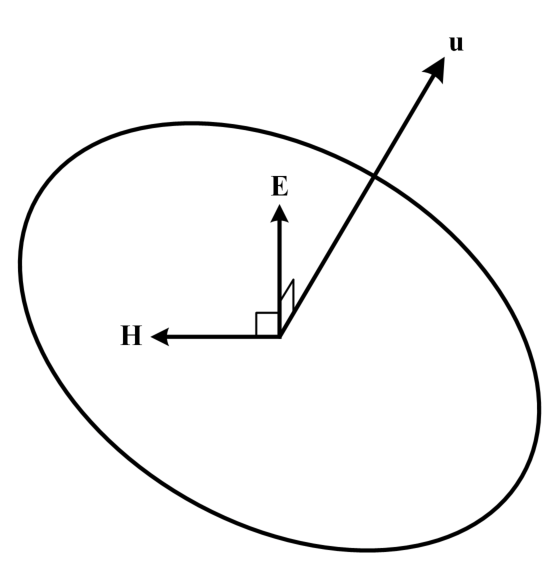
\epsfig{height=2.5in,file=Figs/pw2d/rhs.eps}
		\end{center}
		\caption{Vector fields $\mathbf{E}$ and $\mathbf{H}$ form a right-handed set with $\mathbf{u}$.}
		\label{fig:rhs}
	\end{figure}
	\item [(d)]
	The directions of the vector electric field $\mathbf{E}$, the vector magnetic field $\mathbf{H}$, and the direction of propagation $\mathbf{u}$ are mutually at right angles, as indicated in Fig. \ref{fig:rhs}. The vector $(\mathbf{E},\mathbf{H},\mathbf{u})$ form a right-handed set, which means that they bear the same relationship to each other as, for example, the directions $(\mathbf{u}_x,\mathbf{u}_y,\mathbf{u}_z)$ of the axes of the usual Cartesian coordinate system.\\
\noindent \textbf{Exercise}\\
\noindent Suppose that the above plane wave is traveling in free space in a direction from the origin of a Cartesian coordinate system towards the point (1,1,1), and that we are told that the \textit{x}-component of the electric field has a peak value of $10^{-3}Vm^{-1}$, and that the \textit{y}-component of the electric field is zero. Calculate the remaining field components.\\
\noindent \textbf{Exercise}\\
\noindent Show that for the plane wave described geometrically in Fig. \ref{fig:rhs} the vector magnetic field is given by the vector
	\begin{equation}
	\mathbf{H}=Z^{-1}\mathbf{u} \times \mathbf{E}
	\end{equation}
	\begin{figure}[htbp]
		\begin{center}
			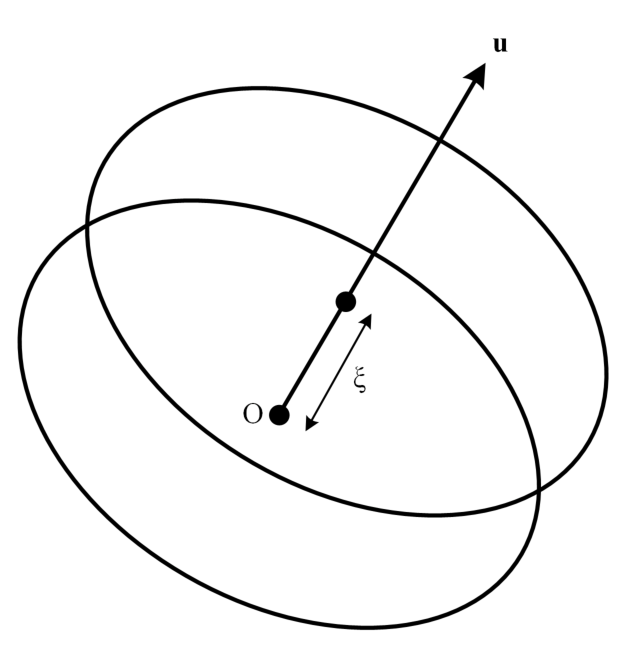
\epsfig{height=2.5in,file=Figs/pw2d/pwpro.eps}
		\end{center}
		\caption{Planes separated by a distance $\xi$ in the direction of propagation.}
		\label{fig:pwpro}
	\end{figure}
	\item [(e)]
	In a lossless medium the magnitude of the fields are the same everywhere but the phase of both the electric and magnetic fields is retarded in the direction of propagation of the wave. Thus, if the electric field over some reference plane containing the point $O$ in Fig. \ref{fig:pwpro}. is $E_0$, then the electric field $E$ over a plane a distance $\xi$ away from the reference plane in the direction of propagation will be
	\begin{equation}
	E=E_0\exp(-jk\xi)
	\end{equation}
	where the time factor $\exp(jwt)$ as is usual for phasor representation of fields, has been suppressed. The phase constant $k$ is the amount by which the phase of the plane wave is retarded in unit distance, and is given by
	\begin{equation}
	k=\omega(\mu\epsilon)^{1/2}
	\end{equation}
	for a lossless medium of permeability $\mu$ and permittivity $\epsilon$. The wavelength $\lambda$ of a propagation wave is the distance over which the phase changes by $2\pi$. Hence
	\begin{equation}
	k=2\pi/\lambda
	\end{equation}
\noindent \textbf{Exercise}\\
\noindent Find the characteristic impedance and speed of travel of a plane wave propagating in a uniform lossless dielectric of relative permeability 1 and relative permittivity 2.56.\\
If now the same dielectric has a small amount of conductivity such that in loss tangent (for a definition see Appendix \ref{sec:promed}) is 0.02 instead of zero, how will this change the characteristic impedance and speed of travel of the plane wave? What is the loss in dB/km?
	\item [(f)] 
	In antenna parlance the term polarization refers to the direction of the vector electric field, which for a plane wave is necessarily confined to planes orthogonal to $\mathbf{u}$. If $\mathbf{E}$ points in a single direction throughout all time and space then the plane wave is said to be \textbf{linearly polarized}. Any plane wave traveling in the direction $\mathbf{u}$ can be represented as the sum of suitable scalar multiples of any two linearly polarized plane waves $\mathbf{E_1}$ and $\mathbf{E_2}$, provided they are not collinear. The most convenient choice is to take $\mathbf{E_1}$ and $\mathbf{E_2}$ to be at right angles, as shown in Fig. \ref{fig:linpol}.
	\begin{figure}[htbp]
		\begin{center}
			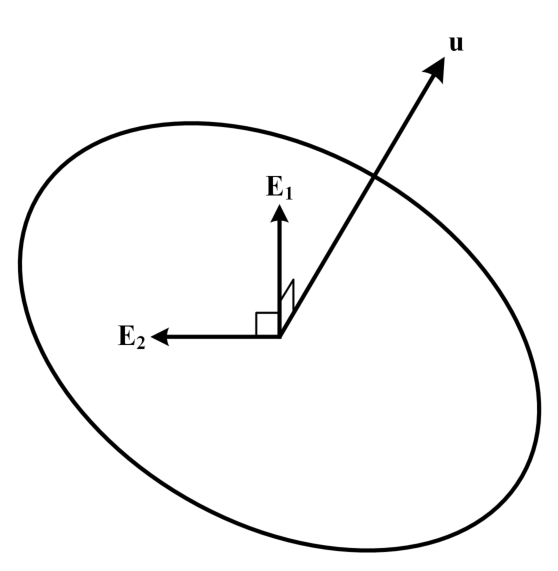
\epsfig{height=2.5in,file=Figs/pw2d/linpol.eps}
		\end{center}
		\caption{Two orthogonal linearly polarized plane waves $\mathbf{E_1}$ and $\mathbf{E_2}$.}
		\label{fig:linpol}
	\end{figure}
	A \textbf{circularly polarized} plane wave is one which can be represented as the sum of two orthogonal linear polarized plane waves of equal amplitude but out of phase by $\pi/2$ radians. Let $\mathbf{E}_1=E_1\mathbf{u}_1$ and $\mathbf{E}_2=E_2\mathbf{u}_2$, where $\mathbf{u}_1$ and $\mathbf{u}_2$ are orthogonal unit vectors, and put $E_1=E_0$ and $E_2=\mp jE_0$. Then the plane wave withe electric field
	\begin{equation}
	\mathbf{E}=E_0\mathbf{u}_1\mp jE_0\mathbf{u}_2
	\end{equation}
	is a circularly polarized plane wave, the negative sign corresponding to clockwise rotation of the electric vector as the wave propagates (also known as right-handed circular polarization), and the positive sign corresponding to anticlockwise rotation (or left-handed circular polarization).\\
	If the two orthogonal linearly polarized plane waves are combine in phase, then the resultant wave is again linearly polarized. The combination of two such orthogonal linearly polarized plane waves is akin to the formation of Lissajou figures on an oscilloscope screen. When their amplitude and relative phases are arbitrary the tip of the electric-field vector traces out an ellipse, and the plane wave is said to be \textbf{elliptically polarized}. (see Appendix \ref{sec:polarization} for a fuller treatment).\\
\noindent \textbf{Exercise}\\
\noindent Show that a linearly polarized plane wave can be represented as the sum of two circularly polarized plane waves traveling in the same direction, of the same amplitude but of opposite sense. Hence show that an arbitrary polarized plane wave can be represented as a suitable weighted sum of two circularly polarized waves of opposite sense.\\
\noindent \textbf{Exercise}\\
\noindent The two linearly polarized electric field vector $\mathbf{E}_1$ and $\mathbf{E}_2$ depicted in Fig. \ref{fig:linpol} satisfy the general orthogonal condition for electromagnetic fields, which is that the scalar product
\begin{equation}
\mathbf{E}_1\cdot{\mathbf{E}_2}^*=0
\end{equation}
in which the asterisk denotes the complex conjugate. Form the two circularly polarized plane waves
\begin{equation}
\mathbf{E}_r=E_1\mathbf{u}_1-jE_1\mathbf{u}_2 \text{ and } \mathbf{E}_l=E_2\mathbf{u}_1-jE_2\mathbf{u}_2
\end{equation}
in which $\mathbf{u}_1$ and $\mathbf{u}_2$ are spatially orthogonal, and show that $\mathbf{E}_r$ and $\mathbf{E}_l$ are themselves orthogonal.\\
	\item [(g)] 
	The power flow in the plane wave is given, as for any electromagnetic wave, by the vector
	\begin{equation}
	\mathbf{E}=\frac{1}{2}\text{ Re }\mathbf{E}\times\mathbf{H}^*
	\label{eq:powflo}
	\end{equation}
	which is the Poynting vector averages over one cycle of the oscillation of frequency $f=2\pi/\omega$. The asterisk denotes complex conjugate and Re the real part. It is clear from Fig. \ref{fig:rhs} that the Poynting vector $\mathbf{S}$ is in the same direction as $\mathbf{u}$, the direction of propagation of the plane wave. The units of $\mathbf{S}$ are watts per square meter. For the homogeneous plane wave of Fig. \ref{fig:rhs} in a lossless medium, the electric and magnetic fields are not only spatially orthogonal but are also precisely in phase, so the vector power flow is
	\begin{equation}
	\mathbf{S}=(2Z)^{-1}|E|^2\mathbf{u}=(Z/2)|H|^2\mathbf{u}
	\end{equation}\\
\noindent \textbf{Exercise}\\
\noindent Rederive the last formula for the power flow in a plane wave by substituting the vector relationship between $\mathbf{E}$ and $\mathbf{H}$, namely.
\begin{equation}
\mathbf{H}=Z^{-1}\mathbf{u}\times\mathbf{E}\text{ or }\mathbf{E}=Z\mathbf{H}\times\mathbf{u}
\end{equation}
into the formula for the average Poynting vector. Use the vector triple product relations for any three vectors $\mathbf{a}$, $\mathbf{b}$ and $\mathbf{c}$, that
\begin{equation}
\begin{aligned}
\mathbf{a}\times(\mathbf{b}\times\mathbf{c})&=(\mathbf{a}\cdot\mathbf{c})\mathbf{b}-(\mathbf{a}\cdot\mathbf{b})\mathbf{c}\\
(\mathbf{a}\times\mathbf{b})\times\mathbf{c}&=(\mathbf{c}\cdot\mathbf{a})\mathbf{b}-(\mathbf{c}\cdot\mathbf{b})\mathbf{a}
\end{aligned}
\end{equation}
\noindent \textbf{Exercise}\\
\noindent Show that the power flow in a plane wave represented as the sum of two orthogonally polarized plane waves is just the sum of the power flows in the two waves.\\
	\begin{figure}[htbp]
		\begin{center}
			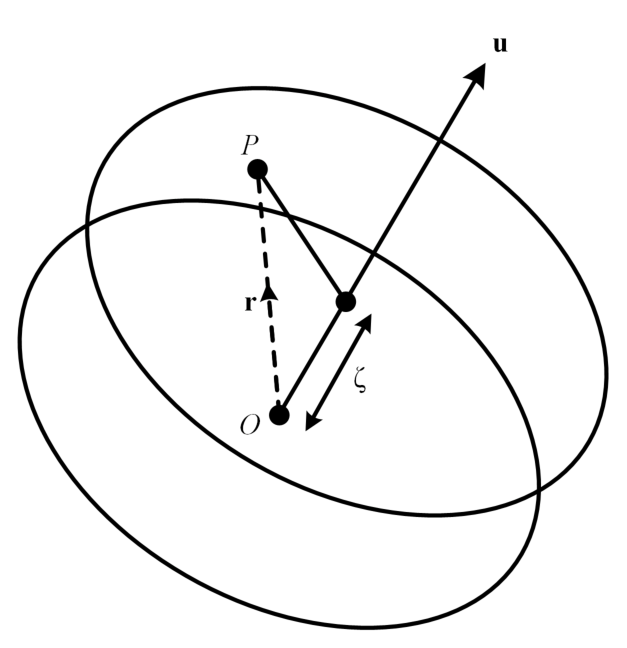
\epsfig{height=2.5in,file=Figs/pw2d/geopw.eps}
		\end{center}
		\caption{Geometry to determine the field at $P$ when a plane wave has electric field $\mathbf{E}_o$ over the plane containing the point $O$.}
		\label{fig:geopw}
	\end{figure}
	\item [(h)]
	Collecting the properties of plane waves given in sections (a) to (g), if a plane wave is propagating in the direction $\mathbf{u}$ in a lossless, uniform isotropic and unbounded medium, and if its vector electric field is $\mathbf{E}_o$ over the plane containing the point $O$ (see Fig. \ref{fig:geopw}), then the vector electric field at the point $P$, whose vector position with respect to the point $O$ is $\mathbf{r}$, will be
	\begin{equation}
	\mathbf{E}(\mathbf{r})=\mathbf{E}_o\exp(-jk\mathbf{u}\cdot\mathbf{r})
	\label{eq:evec}
	\end{equation}
	since the distance between the planes containing $O$ and $P$ is $\zeta=\mathbf{u}\cdot\mathbf{r}$. The electric field, whatever the polarization, must be orthogonal to $\mathbf{u}$, which is expressed by
	\begin{equation}
	\mathbf{u}\cdot\mathbf{E}(\mathbf{r})=0
	\end{equation}
	The vector magnetic field must be orthogonal to both $\mathbf{u}$ and $\mathbf{E}(\mathbf{r})$, and its phasor amplitude is related to that of $\mathbf{E}(\mathbf{r})$ by the characteristic impedance $Z$ of the medium, so that
	\begin{equation}
	\begin{aligned}
	\mathbf{H}(\mathbf{r})&=Z^{-1}\mathbf{u}\times\mathbf{E}(\mathbf{r})\\
	&=Z^{-1}\mathbf{u}\times\mathbf{E}_o\exp(-jk\mathbf{u}\cdot\mathbf{r})
	\end{aligned}
	\end{equation}
	The corresponding expression for the power flow in the plane wave is
	\begin{equation}
	\begin{aligned}
	\mathbf{S}(\mathbf{r})=\frac{1}{2}\text{ Re }\mathbf{E}(\mathbf{r})\times \mathbf{H}^{*}(\mathbf{r})&=\frac{1}{2}\text{ Re }\mathbf{E}_o\times Z^{-1}(\mathbf{u}\times {\mathbf{E}_{o}}^*)\\
	&=(2Z)^{-1}(\mathbf{E}_o\cdot{\mathbf{E}_o^*})\mathbf{u}\\
	&=(2Z)^{-1}|E_o|^2\mathbf{u}
	\end{aligned}
	\end{equation}\\
	Some authors prefer to combine the phase constant $k$ and direction $\mathbf{u}$ into the single quantity
	\begin{equation}
	\mathbf{k}=k\mathbf{u},
	\end{equation}
	sometimes known as the \textbf{vector wavenumber} of the plane wave. It has the virtue of giving information about the frquency (since $k=\omega(\mu\epsilon)^{1/2}$) and direction of the plane wave in one symbol. The electric field at point P is then
	\begin{equation}
	\mathbf{E}(\mathbf{r})=\mathbf{E}_o\exp(-j\mathbf{k}\cdot\mathbf{r})
	\end{equation}
	and similarly for the magnetic field. This slight simplification in the argument of the exponential term is offset by increased complexity elsewhere: in particular, where $\mathbf{u}$ occurs it must be replaced by $\mathbf{k}/k$. We have preferred to retain the explicit dependence of field expression on the direction $\mathbf{u}$, or something equivalent to it, partly for this reason. But the main reason for our choice is to emphasize the fact that the angular plane-wave spectrum, which we are now in a position to examine in detail, is a function of direction.
\end{itemize}

\section{Angular Spectrum for Two-Dimensional Fields}
\begin{figure}[htbp]
	\begin{center}
		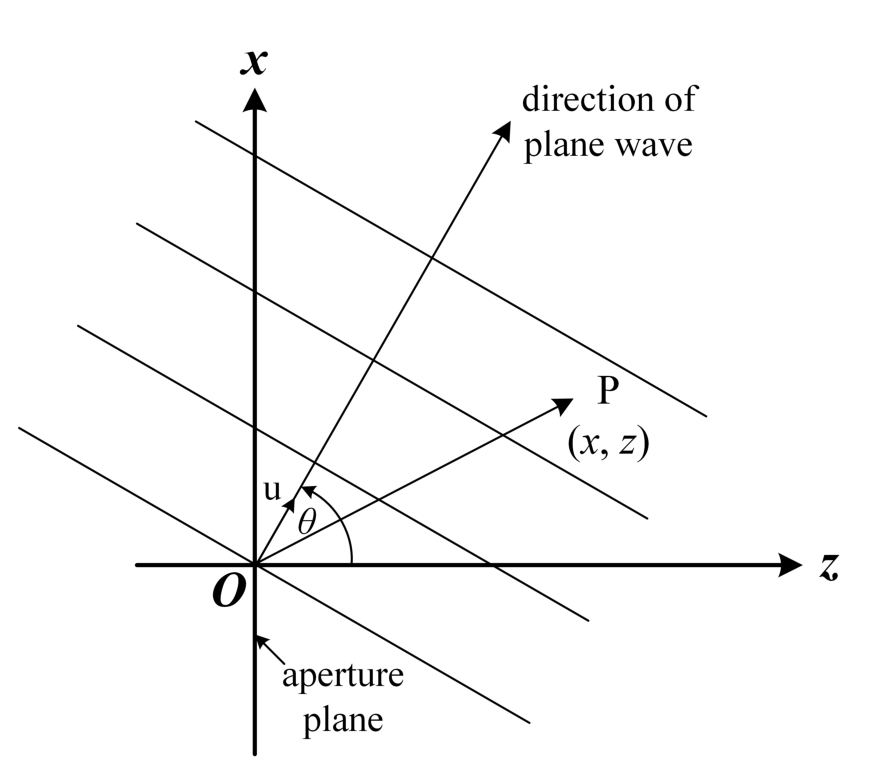
\epsfig{height=2.5in,file=Figs/pw2d/2dgeo.eps}
	\end{center}
	\caption{Two-dimensional geometry for the field which are uniform with $y$, which is at right angles to the plane of the figure.}
	\label{fig:2dgeo}
\end{figure}
Referring to the Cartesian coordinate system of Fig. \ref{fig:2dgeo}, it will be supposed that the fields are uniform with y, and hence depend on the coordinates $(x,z)$ only. The \textit{x}-\textit{y} plane will be taken to be the aperture plane, and our interest will be in the fields diffracted into the supposed uniform, isotropic, source-free and lossless medium to the right of the aperture plane, the half-space $z\geqslant0$.

To construct the fields in this half-space from a set of plane waves traveling in different directions, it is clear that they must all be traveling parallel to the \textit{x}-\textit{z} plane in order that the fields are independent of $y$. A typical member of the set of plane waves is shown in \ref{fig:2dgeo}, its direction \textbf{u} making an angle $\theta$ to the $z$ axis. Since the sources are to the left of the \textit{x}-\textit{y} aperture plane, the plane waves must all travel into the half-space $z\geqslant0$, which restricts $\theta$ to the range
\begin{equation}
-\pi /2\leqslant \theta \leqslant \pi / 2\text{ ,}
\label{eq:trng}
\end{equation}
assuming for now that $\theta$ is real.

The vector position of the field point P with respect to the origin O is
\begin{equation}
\mathbf{r}=\mathbf{u}_xx+\mathbf{u}_zz
\end{equation}
where $\mathbf{u}_x$ and $\mathbf{u}_z$ are unit vectors in the directions of the axes of $x$ and $z$. The unit vector in the direction of propagation of the plane wave is
\begin{equation}
\mathbf{u}=\mathbf{u}_x\sin\theta+\mathbf{u}_z\cos\theta
\end{equation}
Abbreviating this by writing
\begin{equation}
\begin{aligned}
s&=\sin\theta
c&=\cos\theta=\sqrt{1-s^2}
\end{aligned}
\end{equation}
the direction unit vector becomes
\begin{equation}
\mathbf{u}=\mathbf{u}_xs+\mathbf{u}_zc
\end{equation}
in which $s$ and $c$ are the direction cosines. Hence the projection of OP on the direction of the plane wave is
\begin{equation}
\mathbf{u}\cdot\mathbf{r}=sx+cz
\end{equation}

If the vector electric field, as it passes the origin O, is $\mathbf{E_o}$, the electric field at the point P will be
\begin{equation}
\mathbf{E}(x,z)=\mathbf{E}_o\exp{-jk(sx+cz)}
\end{equation}
(see equation (\ref{eq:evec})). It will be convenient to resolve the field into two orthogonal linearly polarized plane waves, one with the electric vector parallel to the \textit{x}-\textit{z} plane and the other with the electric vector perpendicular to the plane. The first of these linearly polarized plane waves has its vector magnetic field pointing entirely in the transverse \textit{y}-direction, and will therefore be referred to as the \textbf{transverse magnetic} (TM) case. The second has its electric field pointing entirely in the transverse direction, and will be referred to as the \textbf{transverse electric} (TE) case. We will treat the TM case first and the TE case, which is simply its dual, later.

\subsection{Angular spectrum of transverse magnetic (TM) fields}
All the plane waves in the angular spectrum which represents a transverse magnetic field in two dimensions will have their electric field lying in the plane of propagation, as depicted in Fig. \ref{fig:tmcase}. The magnetic field will then be wholly transverse.
\begin{figure}[htbp]
	\begin{center}
		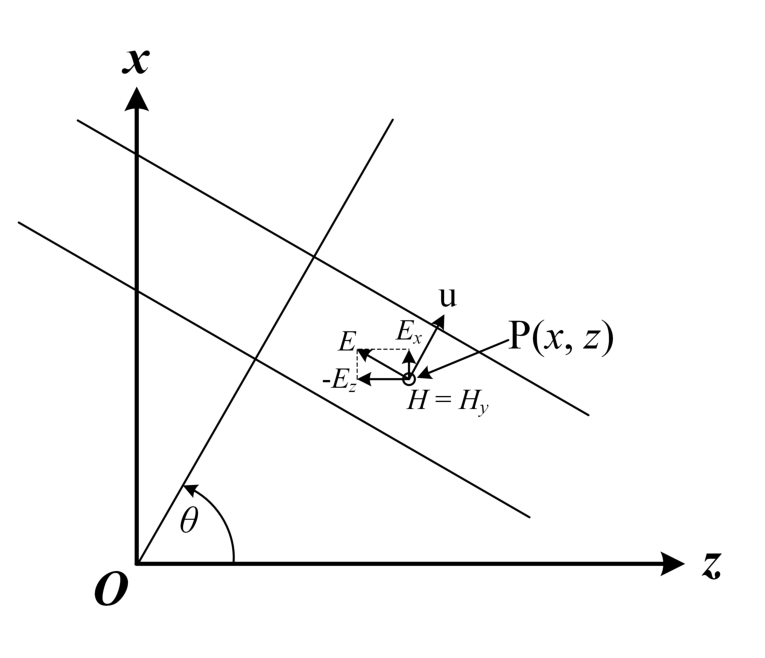
\epsfig{width=3.5in,file=Figs/pw2d/tmcase.eps}
	\end{center}
	\caption{Showing the field components at point P$(x,z)$ for a plane wave whose magnetic field is wholly transverse to the \textit{x}-\textit{z} plane.}
	\label{fig:tmcase}
\end{figure}
If $E_o$ is the phasor amplitude of the electric field of the plane waves as it passes the origin, then the Cartesian components of the electromagnetic field at $\text{P}(x, z)$ will be
\begin{equation}
\begin{aligned}
E_x(x,z)&=E_o\cos\theta\exp{-jk(sx+cz)}\\
E_z(x,z)&=-E_o\sin\theta\exp{-jk(sx+cz)}\\
H_y(x,z)&=Z^{-1}E_o\cos\theta\exp{-jk(sx+cz)}
\end{aligned}
\end{equation}
with the remaining component $E_y$, $H_x$ and $H_z$ all zero. $Z$ is the characteristic impedance and $k$ the phase constant of the medium.

A set of plane waves traveling in different directions is most conveniently represented by a spectrum function $A(\theta)$, such that the electric-field amplitude of the plane wave traveling in the direction $\theta$ is $A(\theta)\mathrm{d}\theta$. This spectrum function is completely analogous to the frequency spectrum function of time-series analysis, and like the frequency spectrum the angular spectrum $A(\theta)$ can be continuous, discrete, or a mixture of the two. The field components are obtained by replacing $E_o$ by $A(\theta)\mathrm{d}\theta$ in the above equation, and then integrating over the range of angles for which the angular spectrum is defined. For example the \textit{x}-component of the electric field will be
\begin{equation}
E_x(x,z)=\int A(\theta)\cos\theta\exp\{-jk(sx+cz)\}\mathrm{d}\theta
\label{eq:asxpol}
\end{equation}
For the reason which will be explained in the next section, it is simpler to express the angular dependence of the spectrum in terms of $s=\sin\theta$, rather than in the terms of $\theta$ itself. So replacing $A(\theta)$ by $F(s)$, and noting that $\mathrm{d}s=\cos\theta\mathrm{d}\theta$, equation (\ref{eq:asxpol}) becomes
\begin{equation}
E_x(x,z)=\int F(s)\exp\{-jk(sx+cz)\}\mathrm{d}s
\end{equation}
which gives the \textit{x}-component of the electric field at the point $(x,z)$ as the integrated effect of all the plane waves in the angular spectrum $F(s)$. Note that $c=\cos\theta$ is retained as a convenient abbreviation for $\sqrt{1-s^2}$.

According to relation (\ref{eq:trng}) the range of integration for $s$ would be $\pm1$. However, it will be shown in the next section that for completeness the $s$ integration has to be extend to cover the whole real line, and hence that the limits of integration for $s$ are $\pm\infty$.

The field components at the point $(x,z)$ for a two-dimensional transverse magnetic field, in terms of the angular plane-wave spectrum function $F(s)$, are therefore
\begin{equation}
\begin{bmatrix}
E_x(x,z)\\
E_z(x,z)\\
H_y(x,z)\\
\end{bmatrix}
=\int_{-\infty}^{\infty}F(s)
\begin{bmatrix}
1\\
-s/c\\
(Zc)^{-1}\\
\end{bmatrix}
\exp\{-jk(sx+cz)\}\mathrm{d}s
\label{eq:3cmp}
\end{equation}
in which $c=\sqrt{1-s^2}$. The important point to note at this stage is that the fields anywhere on and to the right of the aperture plane, that is, in the half-space $z\geqslant0$, have been expressed in the TM case in terms of the single spectrum function $F(s)$. It will be shown later that the remaining field components, which are transverse electric, can be represented by a second spectrum function. But before doing so we will examine some of the important features of the representation of fields by an angular spectrum of plane waves by looking at equation (\ref{eq:3cmp}) in rather more detail.\\
\noindent \textbf{Exercise}\\
\noindent Show by substituting into equation (\ref{eq:3cmp}) that the discrete angular plane-wave  spectrum $F(s)=E_\mathrm{o}c_\mathrm{o}\delta(s-s_\mathrm{o})$, where $s_\mathrm{o}=\sin\theta_\mathrm{o}$, $c_\mathrm{o}=\cos\theta_\mathrm{o}$ and $\delta( )$ is the Dirac delta function, represent a plane wave of amplitude $E_\mathrm{o}$ traveling in the direction $\theta=\theta_\mathrm{o}$.\\
\\
\noindent \textbf{Exercise}\\
\noindent Find the field component of the two-dimensional TM field whose angular spectrum is
\begin{displaymath}
F(s)=\dfrac{E_\mathrm{o}C_\mathrm{o}}{2}[\delta(s-s_\mathrm{o})+s(s+s_\mathrm{o})]
\end{displaymath}
which is in fact the interference pattern of two inclined plane waves of equal amplitude. Sketch the planes of constant amplitude and constant phase. Show, for any of the three field components, that adjacent planes over which its amplitude is zero are separated by a distance $\lambda/(2s_\mathrm{o})$, and that planes of constant phase between which the phase differs by $2\pi$ are separated by $\lambda/c_\mathrm{o}$, where $c_\mathrm{o}=(1-s_\mathrm{o}^2)^{1/2}$.\\
\\
\noindent \textbf{Exercise}\\
\noindent The composite field examined in the previous exercise is of a type known as an \textbf{inhomogeneous plane wave}, since amplitude and phase are both constant over non-coincident planes. Deduce the propagation constant and wave impedance (defined as the ratio of the orthogonal electric and magnetic field transverse to the direction of propagation) of this inhomogeneous plane wave.\\
\\
\noindent \textbf{Exercise}\\
\noindent Determine where, in the fields examined in the previous two exercises, two infinity thin, perfectly conducting, parallel planes may be introduced without disturbing the fields. (See Appendix \ref{sec:wg}, for a fuller discussion, from the point of view of TM modes in a parallel-plate waveguide.)\\
\\
\section{Evanescent Waves}
In order to get a better idea of the physical meaning of the plane-wave spectrum representation of the two-dimensional TM field of equation (\ref{eq:3cmp}), consider the elemental contribution to the \textit{x}-component of the electric field
\begin{equation}
\mathrm{d}E_x(x,z)=F(s)\mathrm{d}s\exp\{-jk(sx+cz)\}
\label{eq:d3cmp}
\end{equation}
which is the contribution of that plane wave in the spectrum of amplitude $F(s)\mathrm{d}s$ traveling in the direction making an angle $\theta=sin^{-1}s$ to the \textit{z} axis.

When $|s|\leqslant1$, $\theta$ lies in the range $-\pi/2\leqslant\theta\leqslant\pi/2$, and the elemental plane wave of equation (\ref{eq:d3cmp}) is of the homogeneous type described in the section \ref{sec:plwa}. The wave travels with characteristic speed of the medium $(\mu\epsilon)^{-1/2}$, and transfers power into the half-space $z\geqslant0$.

But when $|s|>1$, assuming $s$ still to be real, the character of the wave changes because the cosine
\begin{equation}
c=\sqrt{1-s^2}=\pm j\chi \text{  ($\chi$ real and positive)}
\end{equation}
is now imaginary. Substituting this into equation (\ref{eq:d3cmp}), and noting that we must choose $c=-j\chi$ in order that the fields remain finite as $z\rightarrow\pm\infty$,
\begin{equation}
\mathrm{d}E_x(x,z)=F(s)\mathrm{d}s\exp(-jksx)\exp(-k\chi z),
\label{eq:sgtz}
\end{equation}
This is a plane wave of inhomogeneous type, in that the amplitude is no longer constant over planes of constant phase. It has the following properties:
\begin{itemize}
	\item[(a)]
	The direction of propagation of the wave is along the \textit{x}-axis, that is, parallel to the aperture plane, either positive or negative depending on the sign of \textit{s}. The wavefronts over which the phase is constant are shown in Fig. \ref{fig:sgtz}.
	\begin{figure}[htbp]
		\begin{center}
			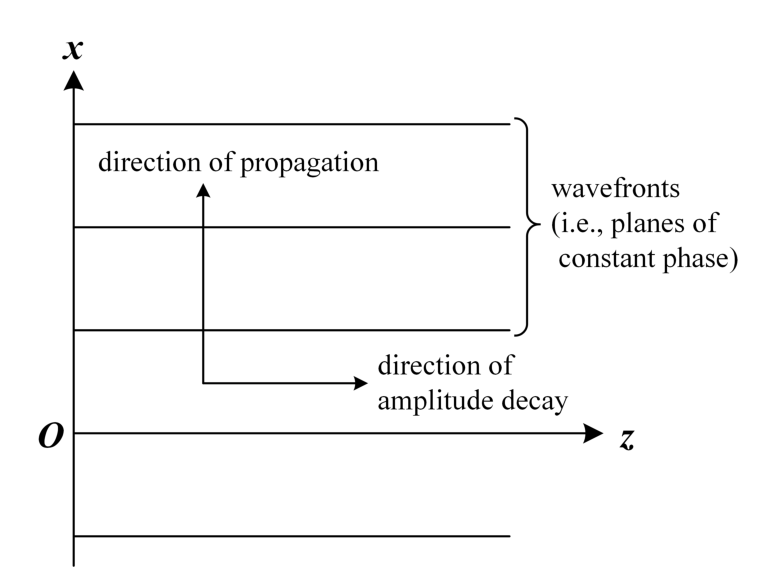
\epsfig{height=2.5in,file=Figs/pw2d/sgtz.eps}
		\end{center}
		\caption{When $|s|>1$ the plane waves of the angular spectrum $F(s)$ are inhomogeneous.}
		\label{fig:sgtz}
	\end{figure}
	\item[(b)]
	The amplitudes of the field components decrease exponentially in the $+z$ direction, away from the aperture plane. For this reason they are often called evanescent, which means disappearing. The distance from the aperture plane at which the amplitude of the elemental plane wave of equation (\ref{eq:sgtz}) has decreased to a fraction $\mathrm{e}^{-1}$ (=0.3679) of its value at $z=0$ is
	\begin{equation}
	z=\dfrac{\lambda}{2\pi\chi}\text{  ,}
	\end{equation}
	where $\chi$ is real and positive. For all but the smallest values of $\chi$ evanescent waves will have become negligibly small at distance of more than a few wavelengths from the aperture plane.
	\item[(c)]
	The phase velocity of the evanescent wave, obtained by restoring the time dependence in equation (\ref{eq:sgtz}), is
	\begin{equation}
	v_p=\dfrac{1}{s(\mu\epsilon)^{1/2}}
	\end{equation}
	This velocity is slower than that of the homogeneous plane waves propagating in the medium, since $|s|>1$. These slow waves do carry power, but it is not propagated into the region $z\geqslant0$. It merely travels back and forth in the aperture plane, and can be thought of as being stored there. Because of their close association with a particular surface, in this case the aperture plane, these waves are also known as electromagnetic surface waves.
\end{itemize}

\noindent \textbf{Exercise}\\
\noindent Use the Poynting vector of equation (\ref{eq:powflo}) to determine the power flow in the elemental wave defined by equation (\ref{eq:d3cmp}) and its associated field components. Compare the two case when $|s|<1$ and $|s|>1$.\\
\\
\noindent \textbf{Exercise}\\
\noindent Define an aperture wave impedance for the elemental wave of equation (\ref{eq:d3cmp}) etc. as
\begin{equation}
Z_{ap}=\dfrac{\mathrm{d}E_x}{\mathrm{d}H_y}
\end{equation}
which is the ratio of the transverse orthogonal components of the electric and magnetic field \textquoteleft looking out\textquoteright\ into the half-space $z\geqslant0$. Show that $Z_{ap}$ is imaginary when $|s|>1$, and comment on the significance of this result.\\
\\
\noindent \textbf{Exercise}\\
\noindent Apply the Poynting vector of equation (\ref{eq:powflo}) directly to the fields of equation (\ref{eq:3cmp}) and show that the total power radiated into the half-space $z\geqslant0$ is
\begin{equation}
P_{rad}=\dfrac{\lambda}{2Z}\int_{-1}^{+1}c^{-1}|F(s)|^2\mathrm{d}s
\end{equation}
It may be useful in achieving this result to note that
\begin{equation}
\int_{-\infty}^{\infty}\exp\{\pm jkx(s-s')\}\mathrm{d}x=\lambda\delta(s-s')
\end{equation}
in which $k=2\pi/\lambda$ and $\delta( )$ is the Dirac delta function.
\begin{figure}[htbp]
	\begin{center}
		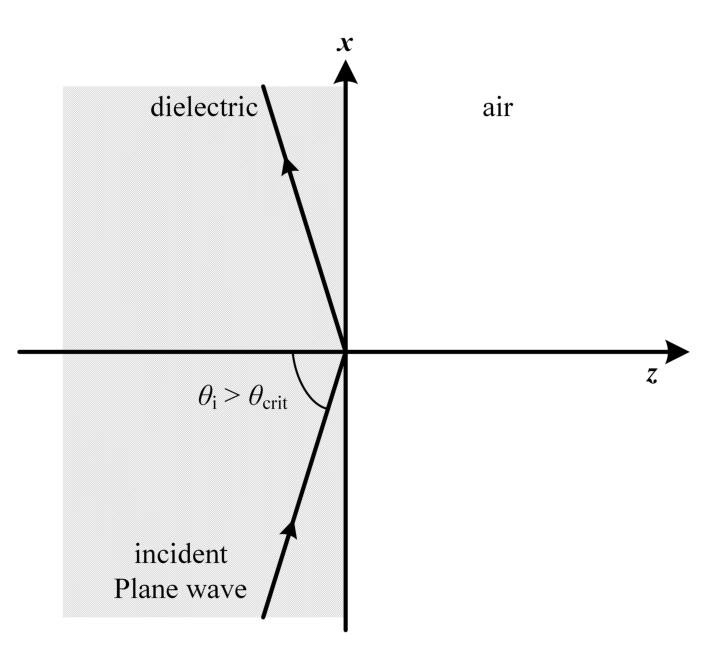
\epsfig{height=2.5in,file=Figs/pw2d/inc2die.eps}
	\end{center}
	\caption{A plane wave incident at a dielectric/air boundary at an angle of incident greater than critical.}
	\label{fig:inc2die}
\end{figure}\\

\noindent{\textbf{Example}}\\
A very instructive physical example of the type of wave we have been discussing occurs on the far side of a dielectric boundary at which total internal reflecting occurs. (see Fig. \ref{fig:inc2die} and Appendix \ref{sec:totref}). In this example the aperture plane will be taken to be coincident with the boundary between the dielectric and air. With a plane wave incident from the dielectric side at an angle of incidence $\theta_i$ greater than the critical angle $\theta_{crit}$ (for which the plane wave transmitted into the air medium would travel in a direction just parallel to the aperture plane) the incident wave will be totally reflected. However, the fields to the right of the aperture plane cannot be zero, since the boundary conditions (see Appendix \ref{subsec:bc}) require that the tangential components of $\mathbf{E}$ and $\mathbf{H}$ be continuous across it. In fact the fields on the air side of the boundary are evanescent waves, which are local to the boundary and carry no energy across it. Thus writing Snell's law as
\begin{equation}
s=\sin\theta_t=(\epsilon_r)^{1/2}\sin\theta_i
\end{equation}
in which $\theta_t$ is the angle of transmission corresponding to the angle of incidence $\theta_i$, and $\epsilon_r$ is the relative permittivity of the dielectric, it is clear that when $\theta_i>\theta_{crit}(=\sin^{-1}(\epsilon_r)^{-1/2})$ $s$ becomes greater than unity but remains real. These are precisely the conditions for which we deduced the properties of evanescent waves.\\

\noindent\textbf{Mathematical Comment}
\noindent What is the nature of $\theta$ when the magnitude of $\sin\theta$ is greater than unity? The answer is that $\theta$ is in general a complex angle. If we apply the two conditions:
\begin{itemize}
	\item [(I)]
	$s$ is real and in the rage $-\infty<s<\infty$
	\item [(II)]\begin{equation}
	\text{when } |s| > 1, c=\sqrt{1-s^2}=-j\chi \text{ is negative imaginary,\linebreak that is, $\chi$ is real and $>$ 0,}
	\end{equation}
\end{itemize}
we can deduce that the contour $\Gamma$ of $\theta$ in the complex-$\theta$ plane, corresponding to $s$ traversing the real line from $-\infty$ to $+\infty$, is that given in Fig. \ref{fig:cplxt}. That par of $\Gamma$ for which $\theta$ is real, namely $-\pi/2\leqslant\theta\leqslant\pi/2$, corresponds to $-1\leqslant s\leqslant1$. The remainder of the contour $\Gamma$ goes off to infinity in directions which ensure that the fields in the angular plane-wave spectrum representation of equation (\ref{eq:3cmp}) are bounded as $z\longrightarrow\infty$.

\begin{figure}[htbp]
	\begin{center}
		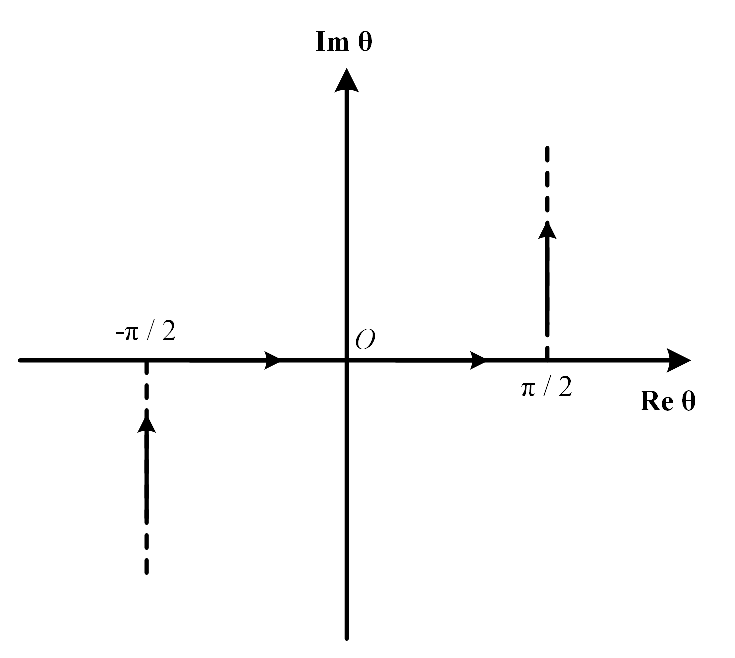
\epsfig{height=2.5in,file=Figs/pw2d/cplxt.eps}
	\end{center}
	\caption{Representation of $\theta$ in the complex-$\theta$ plane: contour $\Gamma$ corresponds to $s=\sin\theta$ tranversing the real line from $-\infty$ to $+\infty$.}
	\label{fig:cplxt}
\end{figure}


\section{Aperture Field: Fourier Transform of the Angular Spectrum}

\section{Far Field: Approximated by the Angular Spectrum}

\section{The Complete Two-Dimensional Field: Uniqueness}











